\chapter{Bent-Core Characterization}
To Do:
- [ ] additional work on homolgous series (do the birefrigence/PRC of PAL29 next
week, so we can include it/get Noel thinking about it.
- [ ] Write list of remaining mysteries (wait until we can get out book)
- [ ] outline characterization section (can't do too much without my harddrive,
but we can look at the paper and supplement and decide where to put the
figures.) Saturday, Dec 29 2018
- [ ]  Read MCLC papers again and memo them for inclusion.
- [ ] Find articles discussing chirality from a mathy and non-mathy perspective,
Saturday, Dec 29 2018
- [ ] A history of de-Vries shit (Carsten's material)

%outline:
%[ ] intro: pick up from the intro, remind the reader about bent-core molecules
%[ ] talk about the homolog series synthesized and summarize previous work
%[ ] talk about PAL30 characterization
%[ ] Remaining mysteries of the PAL30 molecule
%[ ] talk about the other homolog series (additional work needs to be done on
%these)
\section{Introduction and Context}
- Find original synthesis paper
- Talk to Carsten about why they synthesized this phase, so we can include the
motivation.
- Chirality? (I need to think carefully about chirality, and spontaneous
chirality, as this forms a lot of the interesting things about this phase.)
- Time for the knives to come out. Discuss their original PRL paper and
subsequent MCLC, point out all the reasons for their shitty characterization. We
can really go into depth here.

\subsection{Characterization}
-brief summary of characterization before I joined. (Need to decide how in depth
we want to do this i.e. narrative focus, or concise. I'm leaning towards concise
actually. This isn't a history lesson, it is a textbook entry on PAL30. 
-look at Mike's NTB characterization chapter for inspiration here.
\subsection{Modelling}
-talk to Matt about this, how does Spartan work?
-can he recommend a reference that shows how calculating the smectic layer
spacing from this way was actually useful?
\subsection{Optical Texture Analysis}
The optical textures of planar-aligned (bookshelf) cells of
\nfour{phi} were studied using PLM.
Upon cooling from the isotropic, the Sm1 phase grows in (at \SI{175}{\degreeCelsius})
as b\^{a}tonnets, giving a smooth, focal-conic texture typical of an orthogonal fluid smectic (Figure~\ref{fig:main}(f)).
However, given the large value of the estimated
molecular tilt, $\theta_\textrm{xray}$, the Sm1 is probably a de Vries
smectic.
In planar-aligned cells, there is no observable field-induced change of the in-plane birefringence, $\Delta n= n_\parallel
-n_\perp$, in small applied electric fields  (Figure~\ref{fig:main}(f)),
or in the optic axis orientation, $\theta_\text{opt}$ (Figure~\ref{fig:threshold}).

\begin{figure}[h!]
    \centering
    \includegraphics[width=.8\textwidth]{./figs/pal30/finalFigs/shaoresults-v4.png}
    \caption{\label{fig:pal30-texture}Three distinctive optical textures of
        \nfour{phi} at zero field (b,e,h) and with a field applied into (a,d,g)
        and out of (c,f,i) of the plane of the cell. \nt{still have to fix up
    this figure}}
\end{figure}


Below \SI{115}{\degreeCelsius}, a threshold field, $E_\text{th}$, above which a first-order structural change marked by the appearance of chiral conglomerate domains occurs, becomes experimentally accessible.
These domains are polar and exhibit a uniform, saturated optic axis tilt on the
order of $\theta_{\rm opt} \approx \SI{18}{\degree}$ from the layer normal, implying that the achiral, untilted Sm1 phase
transforms in the field to a B2-like, homochiral \smcspf{phi} state (Figure
S1(c))~\cite{eremin2008electrically}. The field-induced left- and right-handed domains form a ``tiger stripe''
pattern (Figures~\ref{fig:main}(e,g)). The local domain handedness in this unusual conglomerate texture 
is apparently locked in after the first few field cycles.  This bias is due to a chiral
memory effect at the surface since, as
Figures~\ref{fig:main}(d)~and~\ref{fig:threshold} show, the
sub-threshold bulk state has an achiral field response, with a linear polarization current (implying $P \propto E$) and no
detectable reorientation of the optical tilt.
$E_\text{th}$  decreases strongly on cooling as the transition to the Sm2 phase is approached, as shown in the inset of Figure~\ref{fig:threshold}.
%
\begin{figure}[h]
    \includegraphics[width=\columnwidth]{./figs/pal30/finalFigs/threshold-inset2.png}
    \caption{\label{fig:threshold}
        Optical tilt of \nfour{phi} vs.\ applied field. The Sm1
        phase shows no electrooptic response in weak fields $E<E_\text{th}$. Fields $E>E_\text{th}$ induce an electroclinic
        tilt and result in the formation of chiral domains.
        $E_\text{th}$, which becomes smaller with decreasing $T$ (inset), matches
        closely $E_\text{sat}$, the field at which the induced
        polarization saturates, extracted from Figure~\ref{fig:main}(d).
        The Sm2 phase exhibits a chiral
        electroclinic effect near $E=0$ and hysteresis in the field-induced helix unwinding to the
        \smcspf{phi} state.   }

\end{figure}


In the lower part of the Sm1, and throughout the Sm2, Sm3 and Sm4 phases, the birefringence increases on application of an electric field, as seen in Figure~\ref{fig:main}(c),  changing from yellow to orange.
Measurements of $\Delta n$ at $E = 0$ and $E = \SI{20}{\volt\per\micro\metre}$
(Figures~\ref{fig:main}(c) and S6),
show that the birefringences in the lower temperature
phases with and without an applied field are of the order of $\Delta n_\text{on} \sim 0.12$ and $\Delta n_\text{off} \sim 0.10$.
Assuming that the field-on \smcspf{phi} state
(Figures~\ref{fig:main}(n--p) and S1) gives a uniform
director orientation with the optic axis in the plane of the cell, then $\Delta
n \sim 0.12$ would correspond to the maximal birefringence $n_3-n_1$ of the
\smcspf{phi} state. Modeling the bent-core molecule
as two uniaxial, birefringent rods connected with an opening angle of
$\Psi$, and tilting this molecule from $z$ by an angle $\theta$,
we have calculated the birefringence of all of the states shown in
Figure~\ref{fig:main}. If the Sm1 phase is assumed to be a de Vries SmA, with
azimuthally averaged molecules distributed on a tilt cone of angle
$\theta$, the best fit to the measured birefringence values $\Delta n_\text{on}$ and $\Delta n_\text{off}$ is
obtained with $\Psi = \SI{150}{\degree}$ and $\theta = \SI{15}{\degree}$.
The calculated birefringence as a function of temperature is shown in Figure~S6.



The transitions between the smectic phases are difficult to see when $E=0$ because they are all orthogonal in appearance,
with an optic axis along $z$, and have similar birefringence.
At the transition from Sm1 to the Sm2 phase,  however, arbitrarily small electric fields induce molecular tilt in the
(Figure~\ref{fig:threshold}), leading to the formation of optically distinct, conglomerate chiral
domains with opposite tilt (Figures~\ref{fig:main}(h--j)), again
corresponding to a field-induced transition to a \smcspf{phi} state.
The birefringence and orthogonal appearance of the Sm2 ground state are consistent with
the helical superlayer structure indicated by RSoXS.

The texture and birefringence of the Sm3 phase in the absence of field are consistent with the \smcapa{phi} bilayer structure indicated by RSoXS.
The field-induced conglomerate domain morphology in both the Sm2 and Sm3 phases is distinct from that of the undulating Sm1
tiger stripes, with straight
domain boundaries that tend to form parallel to the layers, as in an
antiferroelectric calamitic being driven to a ferroelectric
state~\cite{li1995reversible}.
The optical tilt in these domains is found to be $\theta_\mathrm{opt}\sim 18^\circ$.

The response to applied field changes dramatically again at
the transition from Sm3 to Sm4, with no visible brush rotation or evidence of domain formation at any $E$. The birefringence in the Sm4 phase increases continuously with field, saturating
at a value comparable to that observed in the field-induced Sm2 and Sm3 conglomerate domains.

\nfour{phi} transitions into a SmA-like phase from the isotropic phase at
\SI{174}{\degreeCelsius}. This phase is optically confirmed to be smectic as
the smectic layer undulations give rise to characteristic stripes parallel
to the layer normal. These smectic domains grow in as batonnets \nt{fix accent},
 which is again, characteristic to SmA phases. Further cooling results in
 the development of ``tiger stripe'' textures on application of high fields
 (fields larger than some temperature dependent threshold voltage).

 These ``tiger stripe'' textures are unique to the \nfour{phi} molecule, and
 are characterized by wavy undulations of alternating bright and dark
 regions that form parallel to the smectic layers. Though the specific
 dynamics that set the size of these tiger stripes is currently unknown,
 they are thought to form during a transition to chirality, that will be
 discussed in more detail.


\subsection{Polarization Reversal Current}
\begin{figure}[h!]
    \centering
    \includegraphics[width=.8\textwidth]{./figs/pal30/finalFigs/polzv9.png}
    \caption{\label{fig:pal30-prc}Polarization-reversal current of \nfour{phi}.
            A \SI{40}{\hertz} triangular voltage  
                with an amplitude of \SI{72}{\volt} was applied to \nfour{phi} 
                    in a \SI{4.5}{\micro\metre} Instec cell. The voltage
                    zero-crossing
                        is at $t=0$. Three
                            (ferrielectric) current peaks are visible from
                                approximately \SIrange{110}{99}{\degreeCelsius},
                                two
                                    (antiferroelectric) peaks from
                                    \SIrange{99}{83}{\degreeCelsius}, and a
                                        single (ferroelectric) peak from
                                        \SIrange{83}{60}{\degreeCelsius}.
                                            The corresponding liquid crystal
                                            phases are indicated schematically
                                            using
                                            the same color scheme as in Figure
                                            1. Three polarization switching
                                            peaks are understood to
                                            be associated with helical unwinding
                                            (see the discussion of the
                                            SmC$^{*}_\textrm{FI1}$ calamitic
                                            phase in Takazoe et
                                            al.~\cite{takezoe2010antiferroelectric}),
                                            in contrast with the
                                            SmC$^{*}_\alpha$ calamitic phase,
                                            which displays
                                            antiferroelectric (two peak)
                                            behaviour~\cite{lagerwall2005demonstration}.
                                            Though we believe the Sm2 is best
                                            described as an incommensurate
                                            Sm(CP)$_\alpha$ phase, the pitch
                                            ($\approx 2.8$-layer) is much closer
                                            to the $3$-layer
                                            pitch of the SmC$^{*}_\textrm{FI1}$
                                            than the Sm$^{*}_\alpha$ calamitic
                                            phases
                                            (typically 5--50 layers),
                                            which may explain why we see
                                        ferrielectricity.} 
\end{figure}
The polarization reversal current, measured with a triangular
applied field, is shown vs.\ temperature in Figures~\ref{fig:main}(d) and
S7. Upon cooling from the isotropic, a single current bump centered
about $E=0$ first appears at lower temperatures in the Sm1 phase, indicating a Langevin-type
field-induced orientation of $\mathbf{P}$, with a linear response near $E=0$
and the current vanishing  when $\mathbf{P}$ becomes saturated (for $E \ge E_\text{sat}$).
Significantly, $E_\text{sat}$ is similar in magnitude to $E_\text{th}$, the threshold
field required for the Sm1
transition to chirality observed optically (Figure~\ref{fig:threshold}, inset), indicating that the
field first orders the Langevin system of initially azimuthally random molecular
polarizations, with the Sm1 remaining in an achiral state, and that the phase becomes
chiral only at higher fields, once $\mathbf{P}$ is saturated (Figure S8). Upon entering the
Sm2, this polarization bump splits into three peaks roughly centered about
$E=0$, coalescing into two peaks on cooling through the Sm3.
\nfour{phi} thus transforms on cooling from the non-polar
Langevin ground state of the Sm1, where $P=0$ is enforced by entropy, to energetically stabilized ground
states in which the spatial average of
$\mathbf{P}(\mathbf{r})$ in the absence of applied field is also zero: the incommensurate helical winding of the
polarization
in the Sm2, and the antiferroelectric bilayer structure in the Sm3. At the
transition to the Sm4, a single, broad current peak reappears, characteristic of the block
polarization switching of a ferroelectric ground state that is surface-stabilized
with $\mathbf{P}$ parallel to the cell plates at $E=0$, such as occurs in the orthorhombic \smapf{phi} phase~\cite{shen2011effective}.
The absence of brush rotation during the field-induced reorientation of the
polarization in Sm4 is consistent with achiral \smcapf{phi} superlayer organization.

\subsection{X-Ray Scattering}
-- another figure highlighting the tiger stripes
Undoubtably, the most powerful probe in revealing the nanoscale structure of
these phases of matter is light, specifically, light small enough to resolve
this nanoscale structure: X-rays. (digression on Rayleigh resolution/scattering theory?)

For the characterization of PAL30, we used both Small Angle X-ray Scattering
(SAXS) and Resonant Soft X-ray Scattering (RSoXS). For the SAXS, we used the
Synctron Source at ZZ, confirming these diffractograms with a ZZ (in house)
source, shown in Figure XX. 


\nt{include multifig with all the traces on it}

\begin{figure}[h!]
    \centering
    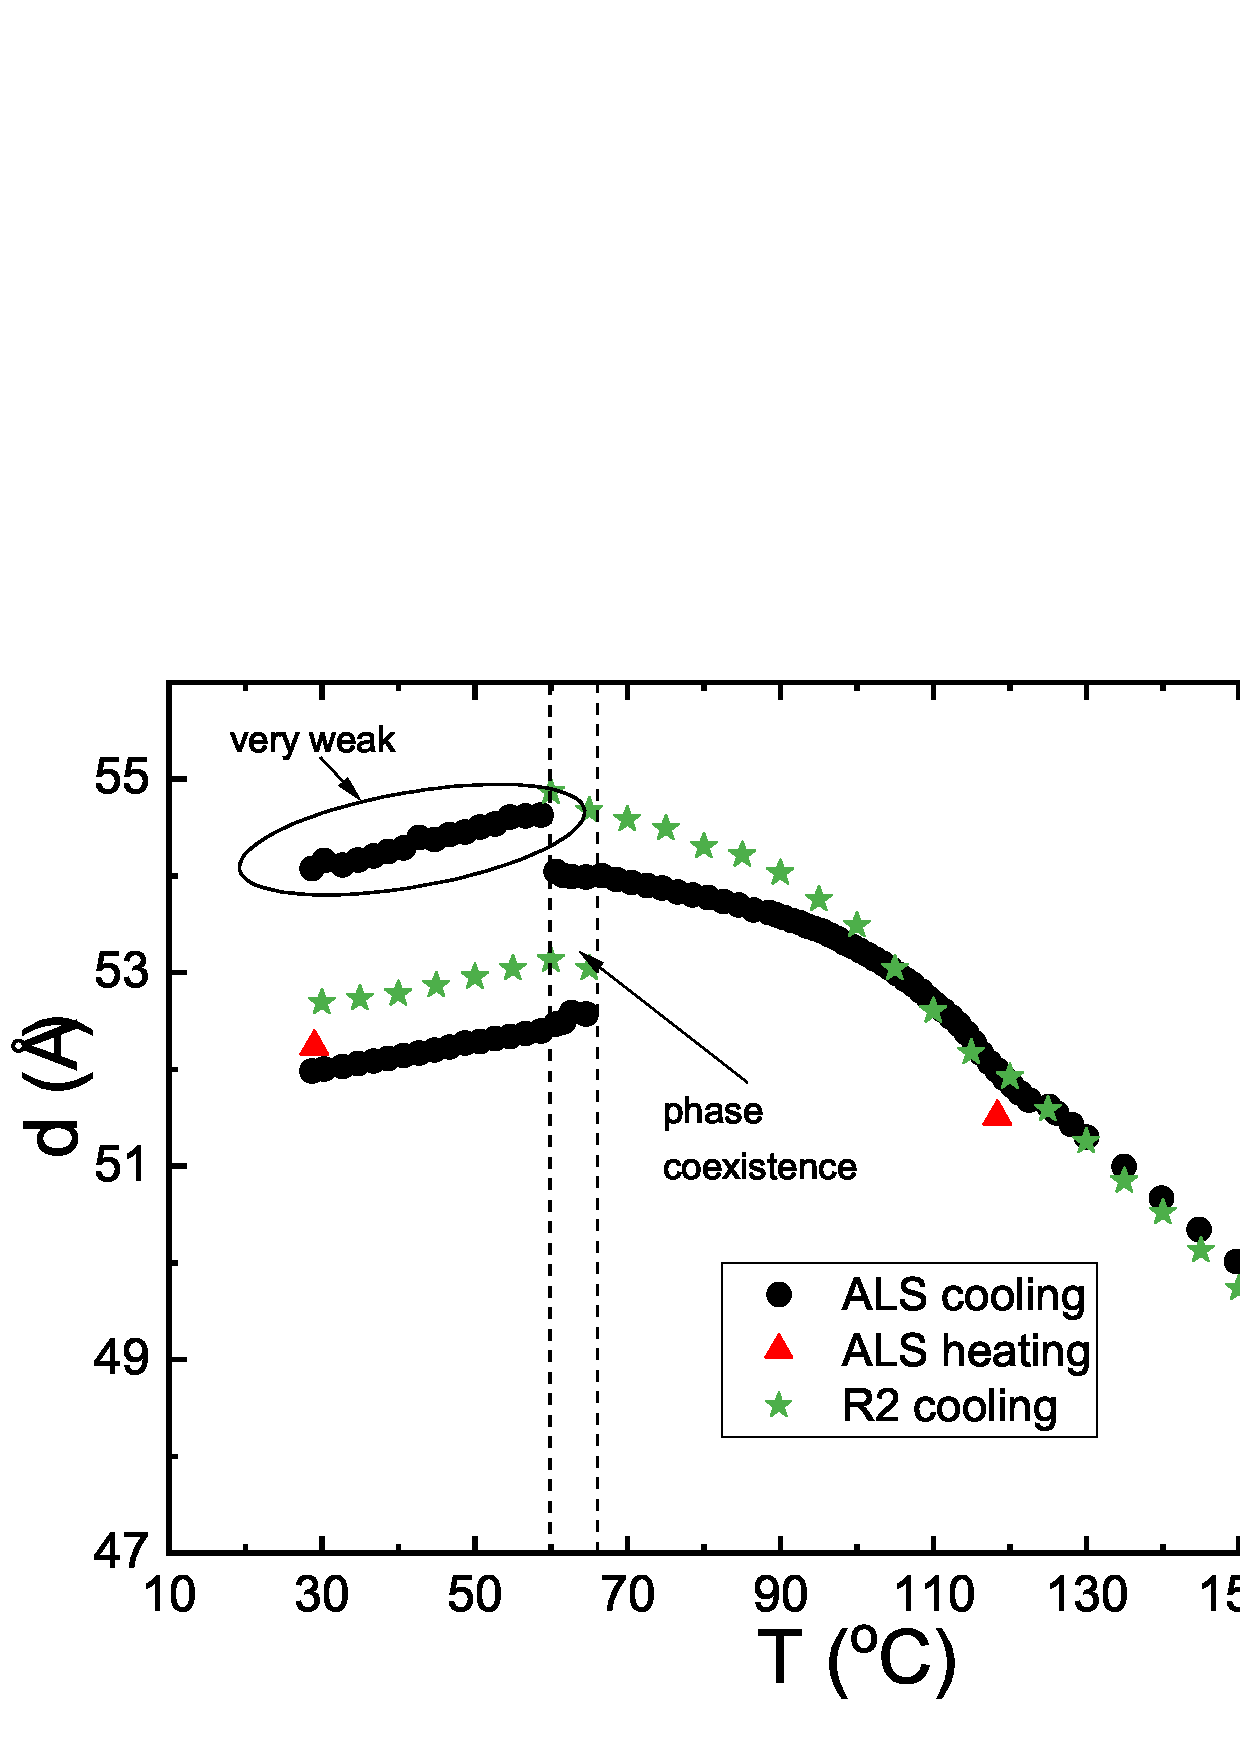
\includegraphics[width=.8\textwidth]{./figs/pal30/finalFigs/combinedALSandR2andAlex.pdf}
    \caption{test}
\end{figure}
As SAXS reveals the underlying electron density structure, it is a powerful,
though oftentimes, blunt tool for revealing the phase structure. For PAL30, we
observed only a single Bragg peak at $\approx \SI{50}{\angstrom}$. The absence
of harmonic peaks indicate that the underlying electron density is very close to
being perfectly sinusoidal, allowing for decomposition into a singular Fourier
wavelength which corresponds to the smectic layer spacing.

%[ ] look at scattering of 8cb (I think Noel mentioned that this was also very
%[ ] What does the height of the peak tell you? Look at old scattering theory
%books (ashcroft)



-include all the SAXS figures, (can we replot them onto the same graph?)
- Discuss smectic layer spacing, talk about what else we can determine from this
-include RSOXS figures (main one).
- orientational at approx $2.8 d_0$, talk about what this could be? Chew the fat
on this one.
\subsection{Resonant Soft X-ray Scattering}
Resonant soft X-ray scattering (RSoXS), as discussed in
Section~\ref{sec:int-rsoxs}, is sensitive to periodicities in the orientation of
the underlying molecules. The RSoXS scans for PAL30 were carried out by Dr.
Michael Tuchband at the Synctron Source in Berkeley.
\nt{include relevant preamble from the supplement about the Berekely facilities}
X-ray scattering from \nfour{phi} is shown in Figures~\ref{fig:main}(b) and S3.
Upon  cooling from the isotropic, a single, non-resonant SAXS peak
appears at $\SI{175}{\degreeCelsius}$, at a wavevector $q_0$  corresponding to Bragg scattering from
the smectic layers in the Sm1 phase with spacing $d_0 = 2\pi/q_0
= \SI{48}{\angstrom}$. The layer spacing increases slightly on cooling
to the crystal phase at \SI{65}{\degreeCelsius} and is
consistently smaller than the calculated molecular length, $l = \SI{59.9}{\angstrom}$, throughout this temperature range, suggesting that the molecules are tilted in all of the smectic phases, to first order by an average amount estimated using $\theta_\textrm{xray} =
\cos(d_0/l)$ of $\SI{33}{\degree}$ (see Figure~S4).
In the Sm1 temperature range ($\SI{110}{\degreeCelsius} \leq T \leq
\SI{175}{\degreeCelsius}$), there are no RSoXS scattering features that would indicate a
superlayer periodic structure (see Figure~S2 and the Supplemental video).

At the transition to the Sm2 phase, at $\SI{110}{\degreeCelsius}$, marked  by
a distinct enthalpy peak in the DSC (Figure~S5
), a single, sharp
resonant peak appears at $q_H = \SI[per-mode=reciprocal]{.042}{\per\angstrom}$, corresponding
to a molecular orientational structure with a period
$d_H=\SI{148}{\angstrom}\approx 2.8 d_0$ that is incommensurate with the
smectic layer spacing (Figure~\ref{fig:xray-results}(b)). Below
$\SI{104}{\degreeCelsius}$, this reflection
becomes weaker and another sharp, resonant reflection at higher $q$ grows in, the coexistence
indicating a first-order transition to the Sm3 phase.
This second Bragg peak, which persists down to the crystal phase, has a
wavevector $q_B\approx q_0/2$, indicative of a commensurate, bilayer orientational
structure in the Sm3 and Sm4 phases.
%
Below \SI{99}{\degreeCelsius}, the incommensurate peak broadens dramatically and
moves to higher $q$, indicating the presence of short-ranged, Sm2-like helical
fluctuations persisting in the Sm3 phase, and disappears at the transition to the Sm4
phase at \SI{83}{\degreeCelsius}. The Sm4 phase exhibits only the bilayer RSoXS
reflection at $q_B$.

\begin{figure}
    \includegraphics[width=\columnwidth]{./figs/pal30/finalFigs/xray-combined.png}
    \caption{\label{fig:xray-results}X-ray scattering from \nfour{phi}.
        (a) SAXS gives a peak from the smectic layer ordering at $q=q_0$.
        The RSoXS peak at $q_H$ indicates that there is superlayer orientational ordering with periodicity $d_H$
        in the Sm2 phase.
        In general, superlayer orientational modulation in a smectic generates RSoXS peaks at wavevectors along the layer normal at
        $q(l,m) = l(2\pi/d_0) \pm m(2\pi/d_H)$\cite{levelut1999tensorial}.  The
        observation of an RSoXS reflection at $q = q(0,1)$ and the absence of an Umklapp peak at $q = q(1,-1)$  in
        the Sm2 confirms a superlayer helix with a scattering amplitude
        modulation due to the smectic layering that is undetectably weak.
        (b) Temperature dependence of resonant scattering. The helix peak at $q_H \approx1/(2.8 d_0)$ becomes diffuse in the Sm3 phase. Splitting
        of the bilayer peak at $q_B$, which would indicate helical precession of the bilayer structure, is not observed.
        }
\end{figure}


The RSoXS scattering from a single layer can be analyzed, following Levelut and
Pansu, in terms of a monoclinic second-rank tensor with a principal
axis tilted from and then azimuthally rotated about the layer normal~\cite{levelut1999tensorial,gleeson_resonant_2006,Barois2012review}.   Scattering
from a stack of such layers is calculated by summing over the contributions of the individual layers at different $z$.
Resonant scattering peaks from azimuthally
periodic arrangements are found at wavevectors along $z$, $q(l,m) = l(2\pi/d_0)
\pm m(2\pi/p)$, where $p$ is the pitch.  In principle, resonant
scattering should appear at all values of $l$ (harmonics of $q_0$), and at values
of $m=0,\pm1,\pm2$ that depend on the superlayer structure.  In an incommensurate, helical
structure, like the SmC$_\alpha$ phase, only the fundamental and harmonic peaks at
$q(l=0,m=+1,+2)$ and the Umklapp peaks at
$q(l=+1,m=-1,-2)$ are found in the range $0 < q(l,m) <
q_0$. If the resonant scatterers are confined to lie precisely on layers spaced
by $d_0$, then the intensities of these peaks will be identical~\cite{levelut1999tensorial}.
Out-of-layer molecular positional fluctuations, and, in particular,
those for which there is a coupled azimuthal orientation that keeps the molecule
on the helix, $\delta \phi = (2\pi/p)\delta z$, reduce the intensities of the
resonant harmonic peak
at $2q_H$ and of the Umklapp peaks at $q_0 \pm q_H$, relative to that of the fundamental at
$q_H$~\cite{levelut1999tensorial}. In our RSoXS scans of these peaks, only the
fundamental is seen above the background, so that only the upper limit of
the intensity ratio of the Umklapp and fundamental peaks
can be estimated. From the RSoXS heating scan of
Figure~\ref{fig:xray-results}(a), we find $I_\text{U}/I_\text{F} \lesssim 0.03$, implying a very
weak fractional modulation of the density of helical scatterers, $\rho$, due to fluctuations in the
smectic layering $\sqrt{\langle\delta\rho^2\rangle}/\rho_0 < 0.17$. The absence of the harmonic peaks places a similar limit on how much the density modulation of helical scatterers deviates from being purely sinusoidal.

\begin{figure}[h!]
    \centering
    \includegraphics[width=.8\textwidth]{./figs/pal30/finalFigs/rsosxSmaT113-modified.png}
	\caption{\label{fig:rsoxs-sm1} Resonant soft X-ray scattering (RSoXS) of \nfour{phi} observed in
        the Sm1 phase ($T=\SI{113}{\degreeCelsius}$). This image is
        characterisitic of the phase. The absence of any
        resonant scattering features is characteristic of the Sm1 showing that
        there are no periodic
    structures present.}
\end{figure}

\begin{figure}[h!]
    \centering
    \includegraphics[width=.8\textwidth]{./figs/pal30/finalFigs/RSoXS-coexistanenceDiffracto.png}
    \caption{\label{fig:rsoxs-coexistDiff} Diffractogram from PAL30 cooling run
        carried out at the Berekely facilities in the coexistance region between
        Sm1 and Sm2. Periodic features are seen at $q\approx
    \SI[per-mode=reciprocal]{.004}{\per\angstrom}$ and $q\approx
\SI[per-mode=reciprocal]{.006}{\per\angstrom}$.}
\end{figure}

These features were confirmed to be resonant peaks by scanning the beam-line
energy through a range, as shown in Figure~\ref{fig:resonant-energy-scan}.
\begin{figure}[h!]
    \centering
    \includegraphics[width=.8\textwidth]{./figs/pal30/finalFigs/resonsnat-energy-scan.png}
    \caption{\label{fig:resonant-energy-scan} The peaks seen at
        \SI{102}{\degreeCelsius} in Figure~\ref{fig:rsoxs-coexistDiff} disappear
        as the beam-line energy is scanned through a range of values, confirming
        that they are resonant, i.e./ they correspond to periodicities in
    \textit{orientation} not \textit{density}.}
\end{figure}

\begin{figure}[h!]
    \centering
    \includegraphics[width=.8\textwidth]{./figs/pal30/finalFigs/PAL30RSOXSshiftedTcontourplotv1mt.png}
    \caption{\label{fig:rsoxs-main} Resonant soft X-ray scattering (RSoXS) of \nfour{phi} observed
        vs.\ temperature on
    cooling. The plot was generated
    from a temperature series of 2D diffractograms that were azimuthally
    averaged, then interpolated and plotted in $q$-space with corresponding real-space coordinates
    ($d=2\pi/q$). Above \SI{110}{\degreeCelsius}, we
    observe no scattering features, indicating the absence of resonant structures periodic in
    this $d$-range. On cooling below \SI{110}{\degreeCelsius}, a scattering arc
    appears at $d=\SI{148}{\angstrom}$, corresponding to  about three smectic layer
    spacings.
    This reflection persists on further cooling but becomes weaker and
    disappears
    at \SI{99}{\degreeCelsius}. At
    \SI{105}{\degreeCelsius}, a second feature appears (at $d =
    \SI{107}{\angstrom}$)
    corresponding to two smectic layer spacings. This feature
    shifts to smaller $q$, and then disappears at the transition to the
    crystal phase at \SI{65}{\degreeCelsius}. In the $q$ range we investigated
    (corresponding to \SIrange{50}{1256}{\angstrom}), we see no other orientational modulations.}
\end{figure}

\begin{figure}[h!]
    \centering
    \includegraphics[width=.8\textwidth]{./figs/pal30/finalFigs/xray-combined.png}
    \caption{\label{fig:xray-combined} X-ray scattering from \nfour{phi}.
        (a) SAXS gives a peak from the smectic layer ordering at $q=q_0$.
        The RSoXS peak at $q_H$ indicates that there is superlayer orientational ordering with periodicity $d_H$
        in the Sm2 phase.
        In general, superlayer orientational modulation in a smectic generates RSoXS peaks at wavevectors along the layer normal at
        $q(l,m) = l(2\pi/d_0) \pm m(2\pi/d_H)$\cite{levelut1999tensorial}.  The
        observation of an RSoXS reflection at $q = q(0,1)$ and the absence of an Umklapp peak at $q = q(1,-1)$  in
        the Sm2 confirms a superlayer helix with a scattering amplitude
        modulation due to the smectic layering that is undetectably weak.
        (b) Temperature dependence of resonant scattering. The helix peak at $q_H \approx1/(2.8 d_0)$ becomes diffuse in the Sm3 phase. Splitting
        of the bilayer peak at $q_B$, which would indicate helical precession of the bilayer structure, is not observed.
        }
    \end{figure}

    \nt{discussion of what this all means, with theory digression to explain the
    flucuations}
\subsection{Comparison to Previous Phases}
\subsection{Remaining Mysteries and Inconsistancies}
-Look at list that I've written down here. (Should work on this firstish, so we
can send it to Leo.)
\section{Homologous Series of PAL30}


